\pagestyle{fancy}
\fancyhead[LE,LO]{OCR A Level - Computer Science NEA}
\fancyhead[RE,RO]{Jonathan Kasongo}

\chapter{Analysis of the problem}

\section{Problem Identification}
% Describe and justify features of the problem that make it 
% solvable by computational methods, explaining why it's 
% amenable to a computational approach.
I aim to write a chess engine capable of beating the 
average chess player at my school 9 times out of 10 for 
one of my classmates John Arco, to learn more about 
strategies in chess and to defeat the best chess players 
in our school.\\

The game of chess has skyrocketed in terms of popularity
recently, so much so that half of my school now spend their
break times playing each other on \url{chess.com}. Chess 
is a strategy board game with the end goal being to checkmate
the opponent's king. \cite{rules} This means that capture of 
the opponent's king is inevitable upon the next move. The 
game also involves \textit{no} elements of luck and the 
outcome of the game is soley dependent on the actions of the
player. Moreover, the game of chess is known to be very
hard to master with many of the best chess
\textit{Grandmasters} starting training from the
ages of 7-8 \cite{Magnus}. The game of chess has an average
of 35 moves \cite{branch} per position. This means that 
if one wants to think three moves ahead of his opponent
he must consider $42,875$ positions in total! This is
simply not possible for a human, however for a computer
this task is something that could be done in less than
1 second. By leveraging the high computational power
of modern computers, I aim to write a chess engine that
is able to beat an average human chess player 9 times
out of 10.\\

Whilst chess prodigies and Grandmasters dedicate their entire
lifes to improving their chess abilities, using high order 
thinking processes, experience and strategical tactics to play
the best move in a position we may simply use a "brute-force" 
style of searching, in which we consider all legal moves from a 
given position and simply choose the one that gives the most
advantageous position even if our opponent plays the best 
responses each time. Claude Shannon \cite{shan} identified 2 main
categories of search algorithms. \cite{search} 

\begin{itemize}
  \item{Type A - A brute-force search looking at every variation
        to a given depth.}
  \item{Type B - A selective search looking at important variations 
        only.}
\end{itemize}

According to Shannon, this is model will fall into a
type A search. Though type B searches look at less variations and 
are therefore faster, I argue that type A searches are more sustainable 
today with the speed of modern computers. This allows us to consider all 
variations without having a massive performance hit to our program.\\

For each move that we consider, there is a number of 
responses that our opponent can make, similarly for each of 
\textit{those} moves we also have a number of possible 
responses to consider. This gives us a \textit{search tree}
in which each node is a move to consider and each of the 
child nodes are possible responses to the played move. A 
simple visualisation of this can be seen below.\\

Consider the opening move from white, e4
\footnote{Evaluations are from Stockfish 14 NNUE.}

% Useful document on how to draw game trees with Tikz
% https://www.sfu.ca/~haiyunc/notes/Game_Trees_with_TikZ.pdf
\begin{center}
  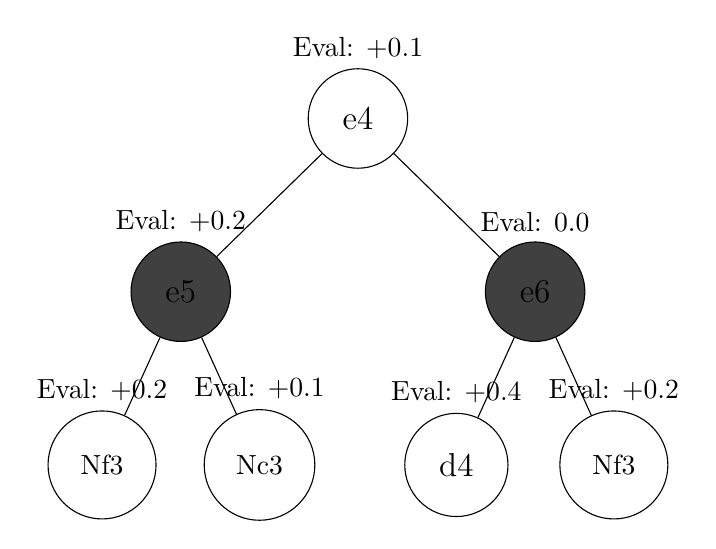
\begin{tikzpicture}[level 1/.style={sibling distance=4.5cm},level 2/.style={sibling distance=2cm}]
  \tikzstyle{w}=[circle,draw,inner sep=8]
  \tikzstyle{b}=[circle,draw,inner sep=8,fill=darkgray]
  
  \node[w,label=above:{Eval: +0.1}]{\large e4}
    child{node[b,label=above:{Eval: +0.2},yshift=-0.7cm]{\large e5}
      child{node[w,label=above:{Eval: +0.2},yshift=-0.7cm]{Nf3}}
      child{node[w,label=above:{Eval: +0.1},yshift=-0.7cm]{Nc3}}
    }
    child{node[b,label=above:{Eval: 0.0},yshift=-0.7cm]{\large e6}
      child{node[w,label=above:{Eval: +0.4},yshift=-0.7cm]{\large d4}}
      child{node[w,label=above:{Eval: +0.2},yshift=-0.7cm]{Nf3}}
    };
\end{tikzpicture}
\end{center}

This is one possible search tree that we could look at. This
tree is only considering 2 moves for white and black, 
however in reality there is usually much more moves to 
consider per position. To traverse this tree we would start
at the e4 node at the top. We would then move to the e6 node
because this gives the better evaluation for black (black 
wants to minimise evaluation and white wants to maximise it).
Then white will choose to play d4 in this position because
it gives a higher evaluation $(0.4>0.2)$. Now even if black 
plays the best move in the original starting position: e6 
we know that we have an adequate response that will bring 
evaluation in our favour! Namely we will respond with d4.

The problem of traversing a tree with directed edges is one
that has been heavily researched in computer science and is 
a principal component in the programming of any chess engine.
Moreover, the strategical nature of the game coupled 
with the fact that it has a high branching factor makes this
problem amenable to a computational approach.


\section{Stakeholders}
% https://www.nytimes.com/2022/06/17/crosswords/chess/chess-is-booming.html
% Identify suitable stakeholders for the project and describe how will make
% use of the proposed solution and how it is appropiate to your needs.
One of the students at my school who plays chess regularly is 
John Arco. John Arco is a 17 year old male with a passion for chess.
John has a rating of roughly 1000 ELO but wishes 
to improve to a higher rating and beat all of his 
classmates. John is also very competitive and wishes to 
\textit{guarentee} that none of his classmates can beat him.
The use of a strong chess engine is one method to ensure
that John Arco always beats his classmates and requires little
to no effort on his part, all he has to do is replicate the 
moves played by his opponent on the engine's board and he 
will simply replicate the computer's moves. 
\footnote{I do realise that this is considered cheating,
however we intend to use this engine completely offline
in unrated friendly games against close friends. 
I do not advocate cheating in any way shape or form.}
Moreover using a chess engine can also be highly educational as
we may learn new ideas or moves from the engine that we may have
never considered previously. Even Magnus Carlsen
has openly said that he has learnt new ideas from chess engines.
\cite{lex} This means the engine is to serve 2 purposes,
the first is ensure that John Arco remains undefeated 
against his classmates, and the second is to improve John Arco's
chess ability by exposing him to new and unique tactics that 
he wouldn't have thought of otherwise. The construction of 
a strong chess engine will be able to solve both problems
effectively, providing both educational benefits and 
competitive benefits also. \par

The following is a transcript of an interview I
conducted with my client John Arco on how he will make use of the
engine and how it is appropiate to his needs. This will 
help me to clearly understand the requirements and goals I
should keep in mind when programming.\\

\begin{tcolorbox}
\makebox[2cm]{\textbf{Jonathan:}} Why are you looking for a chess engine?\par
\makebox[2cm]{\textbf{John:}} I am looking to improve my
chess rating to around 2000 ELO, and a chess engine would
help me a lot.\par
\makebox[2cm]{\textbf{Jonathan:}} What features should this
engine have? \par
\makebox[2cm]{\textbf{John:}} The engine should definitely
play at a strength stronger than me, It should also include
an easy to use GUI and it can be written in any programming
language.\par
\makebox[2cm]{\textbf{Jonathan:}} How will you use the
engine? \par
\makebox[2cm]{\textbf{John:}} I will play games against the 
engine to practise and improve my rating, I will also use it
to review my games to help me see the mistakes in the moves 
that I played. \par
\makebox[2cm]{\textbf{Jonathan:}} How will the engine be 
appropiate to your needs? \par
\makebox[2cm]{\textbf{John:}} This engine will allow me to 
easily analyse my games from my laptop, and help me in 
achieving my goal of chess mastery in the process.
\end{tcolorbox}

\subsection*{Analysis of interview}
Based on the interview with my client I was able to get 
some clear features, that the finished program should
include. The request to have the engine play at a strength
of >1000 ELO, is no simple task so it will be split into
numerous sub-tasks that will aid me in designing the final 
program. \\

\textbf{\large Requirement list:}
\begin{itemize}
  \item Be easy to use
  \item Include a clean user interface
  \item Play at a strength of <1000 ELO

  \begin{itemize}
    \item{Generate legal moves with a consistent and fast
          algorithm}
    \item Evaluate positions with heuristical optimisations
    \item{Search for moves with a suitable algorithm}
  \end{itemize}

\end{itemize}

\section{Research the problem}
The following subsections will act to be 
a brief summary of the research I conducted on understanding
how to write a chess engine.\\

Any chess engine must be comprised of these 3 fundamental components:
\begin{itemize}
  \item \textit{Legal move generation}
  \item \textit{Evaluation functions}
  \item \textit{Searching algorithms}\\
\end{itemize}

We will explore each of these components in detail, however 
if you have never come across the term "bitboards" in 
relation to chess programming, I strongly 
encourage you to read the next subsection.

\subsection*{Bitboards}
To understand the following algorithms it is nescessary to 
have an adequate understanding on \textbf{\textit{bitboards}}.
If you already understand this concept please skip this 
subsection entirely, otherwise I will provide a brief 
introduction to the idea here. Some helpful resources can be
found here \cite{bitboards}.\\

Every chess engine needs a way to represent the state of the
chess board. Bitboards are one such way to represent the
state of the chess board with 64 bit integers. Consider
the following chess position.

\begin{figure}[h]
  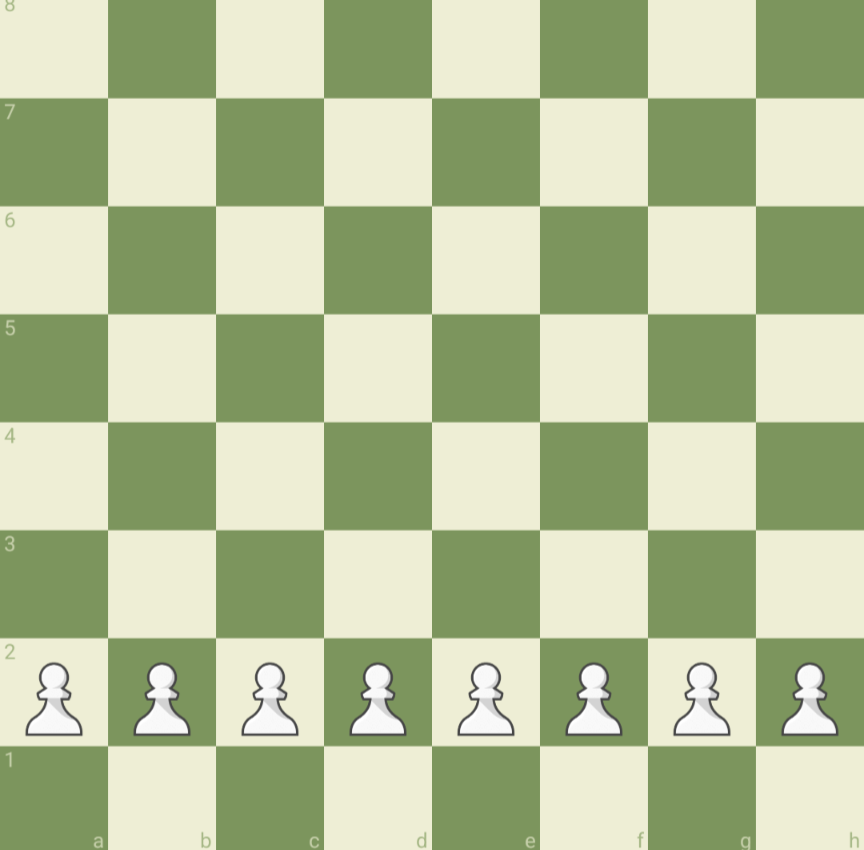
\includegraphics[scale=0.25]{White_Pawns_start.png}
  \centering
  \caption{Starting position for white pawns}
  \label{whitepawns}
\end{figure}

Immediately we may notice that a chess board has dimensions
$(8 \, \textrm{x} \, 8)$ and 64 squares. Furthermore, 
each of the squares in figure \ref{whitepawns} exists 
in one of these two states: There either is a white pawn on
this square or there is not. Does this remind you of a 
familiar concept in computer science? This innate similarity to 
the binary numbering system motivates one to consider the 
use of binary in order to represent a chess board. We can take a 
64 bit unsigned integer and have each \texttt{0} 
represent the lack of a piece and similarly 
have each \texttt{1} represent the existance of a piece on 
this square.\\

Consider the following code snippet.\footnote{The importing
of the numpy library has been omitted for clarity.}

\begin{minted}[linenos, bgcolor=lightgray]{Python}
  # For the rest of this paper i64 will refer to the 
  # unsigned 64 bit integer
  i64 = np.uint64
  WhitePawn = i64(0b        # Dots represent 0,
                  00000000  # . . . . . . . .
                  00000000  # . . . . . . . .
                  00000000  # . . . . . . . .
                  00000000  # . . . . . . . .
                  00000000  # . . . . . . . .
                  00000000  # . . . . . . . .
                  11111111  # 1 1 1 1 1 1 1 1
                  00000000) # . . . . . . . .
\end{minted}

Each bit in the \texttt{WhitePawn} variable represents the
state of a square like we saw previously, this allows us to 
store the state of the board with 12, 64 bit numbers 
(6 piece types in chess, and 2 players). Modern computers
typically have register sizes of 64 bits or greater, 
meaning that we may easily and quickly manipulate these 
bitboards in order to generate legal moves for a position.
We will consider how we may leverage bitboards for legal 
move generation in the following subsection. 
\footnote{We assume reverse little endian indexing for 
our boards throughout.}

\subsection*{Legal move generation}
Legal move generation is the first step to writing a strong
chess engine, in this component we wish to 
find a way to feed in a position to a computer program and have it 
output to us all of the possible legal moves available in this position.
The study of move generation algorithms in the chess programming world 
is still very nascant, with one of the newest algorithms
being discovered in 2017 \cite{bm}. The two algorithms I
decided to spend time researching were
\textit{Hyperbola quintessence} and 
\textit{Magic bitboards} because they are the standard 
accepted algorithms for the top chess engines 
\cite{stockfish}. Both these algorithms are used to generate
moves for sliding pieces 
\footnote{That is the queen, bishop and rook.}.\\

\subsection*{Magic bitboards}
Magic bitboards were discovered in 2006 by Lasse Hansen
\cite{lasse}, and was heavily influenced by Gerd Isenberg's
\textit{"Kindergarten"} bitboards. Both techniques use the
same core idea: we will access moves from a pre-initialised
moves array/table instead of calculating the required move
set on the fly. Magic bitboards involves the usage of a 
\textit{perfect} hash function to map all possible board
occupancies to all their corresponding move sets. By 
occupancy I mean some bitboard of all other pieces that
are able to block the movement of our sliding piece. For 
instance consider a rook on the A1 square, if there is 
another piece on the D1 square the rook will not be able to 
move past D1 anymore. After we hash our occupancy bitboard,
we will use it to index into a pre-calculated attack array
that will give us a bitboard of the correct legal moves in 
$O(1)$ time and space complexity. Examples are often the 
best way to explain concepts so let's go through a simple one.
Let's use our rook that was on A1. It's bitboard will look 
like this:

\newpage
\begin{minted}[linenos, bgcolor=lightgray]{Python}
  WhiteRook = i64(0b        # Dots represent 0,
                  00000000  # 8 |. . . . . . . .
                  00000000  # 7 |. . . . . . . .
                  00000000  # 6 |. . . . . . . .
                  00000000  # 5 |. . . . . . . .
                  00000000  # 4 |. . . . . . . .
                  00000000  # 3 |. . . . . . . .
                  00000000  # 2 |. . . . . . . .
                  10000000) # 1 |1 . . . . . . .
                            #    _______________
                            #    A B C D E F G H
\end{minted}

The technique is no doubt fast, we are simply accessing
an array, the concern with this technique is rather it's
memory consumption.

\subsection*{Hyperbola quintessence}
